\paragraph{}This chapter goes over 2 examples of tuning 2 distinct \ac{SLAM} algorithms(faster-lio and fast-livo2), using all three tuning algorithms implemented. Given that the purpose of this dissertation is to optimize \ac{SLAM} solutions, there is not much sense in comparing the effectiveness of faster-lio and fast-livo2. It was therefore decided that the focus of this section should instead be on showcasing the implemented tuning algorithms, according to a predefined tuning strategy.

%So, it was decided to optimize each of these algorithms for a different metric, aligning the optimization goal with the algorithm's design goals. faster-lio was optimized for \ac{RPE}, while fast-livo2 was optimized for \ac{APE}.

\section{faster-lio}

\paragraph{}It is important, before tuning any hyperparameter, to run the algorithm with default parameters, to know what the \ac{RPE} is when no optimization is performed. Below is a table with the 5 run average of the \ac{APE} and \ac{RPE} for the faster-lio algorithm(table \ref{default-faster-lio}). These results were obtained with the parameter values specified in table

\begin{table}[h]
\centering
\begin{tabular}{|l|l|}
\hline
APE(RMSE) & RPE(RMSE) \\ \hline
0.664834  & 0.015037  \\ \hline
\end{tabular}
\caption{Default parameter results(5 run average) for faster-lio}
\label{default-faster-lio}
\end{table}

\begin{table}[]
\centering
\begin{tabular}{|l|l|}
\hline
point\_filter\_num     & 3    \\ \hline
max\_iteration         & 3    \\ \hline
filter\_size\_map      & 0.5  \\ \hline
filter\_size\_surf     & 0.5  \\ \hline
cube\_side\_length     & 1000 \\ \hline
ivox\_grid\_resolution & 0.5  \\ \hline
esti\_plane\_threshold & 0.1  \\ \hline
\end{tabular}
\caption{Default parameter values for faster-lio}
\label{default-faster-lio-params}
\end{table}

\paragraph{}Before running Simulated Annealing, it is necessary to define the hyperparameters of the algorithm.

\paragraph{}Then, the following parameter space was devised. The below two tables show the configuration of the optimized faster-lio parameters for simulated annealing. They are separated into two tables: one for discrete parameters and one for continuous parameters.

\begin{table}[h]
\centering
\begin{tabular}{|c|c|c|c|c|}
\hline
Parameter          & Initial Value & Lower Bound & Upper Bound & delta max \\ \hline
point\_filter\_num & 20            & 2           & 50          & 8         \\ \hline
max\_iteration     & 10            & 3           & 50          & 5         \\ \hline
cube\_side\_length & 1100          & 700         & 2000        & 300       \\ \hline
\end{tabular}
\caption{faster-lio discrete parameter settings}
\label{faster-lio-discrete-params-settings}
\end{table}

\begin{table}[h]
\centering
\begin{tabular}{|c|c|c|c|c|c|}
\hline
Parameter              & Initial Value & Lower Bound & Upper Bound & $\mu$     & $\sigma$     \\ \hline
filter\_size\_map      & 0.5           & 0.1         & 0.75        & -0.01 & 0.003 \\ \hline
filter\_size\_surf     & 1.0           & 0.25        & 1.25        & -0.01 & 0.003 \\ \hline
ivox\_grid\_resolution & 0.5           & 0.1         & 0.75        & -0.01 & 0.003 \\ \hline
esti\_plane\_threshold & 0.5           & 0.1         & 0.75        & -0.01 & 0.003 \\ \hline
\end{tabular}
\caption{faster-lio continuous parameter settings}
\label{faster-lio-continuous-params-settings}
\end{table}

\begin{figure}[h]
    \centering
    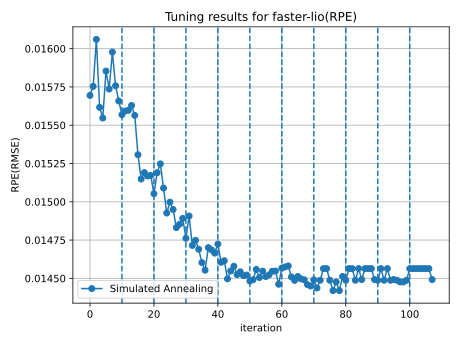
\includegraphics[width=0.65\linewidth]{images/faster-lio-sa.pdf}
    \caption{RPE per iteration of Simulated Annealing}
    \label{faster-lio-sa}
\end{figure}

\paragraph{}The vertical dotted lines represent the iterations where the temperature was reset to its initial value(reannealing). 

\paragraph{}From figure \ref{faster-lio-sa}, it can be seen that, roughly for the first 80 iterations, reannealing allows the algorithm to escape a local minima and achieve a better solution than the incumbent. After that, it gets stuck and doesn't go anywhere for almost 30 iterations, which was the limit proposed for halting the execution, when no better solution is found. This parameter is customizable, but it was decided, after a few runs with a 30 second section of the dataset, that it was not productive to let the algorithm run for so long without achieving any better solution. Also, given the time each Simulated Annealing run takes(2.5 minutes x ([50, 100] iterations) = [2, 5] hours), some shortcuts had to be taken. One was that most optimizations, in terms of parameter settings, such as delta\_max for discrete parameters or gaussian curve $\mu$ and $\sigma$ values for continuous parameters were adjusted while working with 30 second sections of the dataset. While it does not guarantee that such adjustments will work on the entire dataset, it allows the researcher to understand how their values affect algorithm runtime and performance.

\begin{figure}[h]
    \centering
    \includegraphics[width=0.75\linewidth]{images/cube_side_length_rpe.pdf}
    \caption{cube\_side\_length scatter plot}
    \label{cube_side_length_scatter}
\end{figure}

\paragraph{}Figure \ref{cube_side_length_scatter} shows the scatter plot for the discrete parameter. It indicates the optimal range for this parameter is between 1300 and 1700. This isn't conclusive, however. Correlation does not mean causation. Other parameters were tuned and their effects on the \ac{RPE} may be greater, such as filter\_size\_surf(figure \ref{filter_size_surf_scatter}) and ivox\_grid\_resolution(figure \ref{ivox_grid_resolution_scatter}). In both cases, the relationship between parameter value and the \ac{RPE} is even clearer. For these two parameters, the lower their values, the lower the \ac{RPE}. Although filter\_size\_surf seems to stabilize for values between 0.25 and 0.5, it was decided to explore even lower values. For ivox\_grid\_resolution, the lower bound was defined as 0.1, hence why there weren't any values below it. Even though there the scatter plot shows a possible linear relationship between this parameter and the \ac{RPE}, it might be worthwhile to explore lower ivox\_grid\_resolution values. For the parameters filter\_size\_map and esti\_plane\_threshold, the scatter plots looked very similar to filter\_size\_surf and ivox\_grid\_resolution, and a similar reasoning regarding further optimization was applied.

\begin{figure}[h]
    \centering
    \includegraphics[width=0.65\linewidth]{images/filter_size_surf_rpe.pdf}
    \caption{filter\_size\_surf scatter plot}
    \label{filter_size_surf_scatter}
\end{figure}

\begin{figure}[h]
    \centering
    \includegraphics[width=0.65\linewidth]{images/ivox_grid_resolution_rpe.pdf}
    \caption{ivox\_grid\_resolution scatter plot}
    \label{ivox_grid_resolution_scatter}
\end{figure}

\paragraph{}After analyzing the scatter plots, the parameter space to be explored further using Grid Search and Random Search is the following:

\begin{table}[h]
\centering
\begin{tabular}{|c|c|c|c|}
\hline
Parameter              & Initial value & Step size & Number of values \\ \hline
cube\_side\_length     & 700           & -         & 1                \\ \hline
max\_iteration         & 15            & -         & 1                \\ \hline
point\_filter\_num     & 4             & -         & 1                \\ \hline
esti\_plane\_threshold & 0.01          & 0.01      & 10               \\ \hline
filter\_size\_map      & 0.01          & 0.01      & 10               \\ \hline
filter\_size\_surf     & 0.15          & 0.01      & 11               \\ \hline
ivox\_grid\_resolution & 0.01          & 0.01      & 10               \\ \hline
\end{tabular}
\caption{faster-lio grid/random search parameter space}
\label{faster-lio-parameter space}
\end{table}

\subsection{Grid Search}

\paragraph{}Grid Search was run for 5 hours. Its \ac{RPE} per iterations is shown in the figure below(figure \ref{faster-lio-grid-search-rpe}).

\begin{figure}[h]
    \centering
    \includegraphics[width=0.75\linewidth]{images/faster-lio-grid-search-rpe.pdf}
    \caption{RPE per iterations of Grid Search}
    \label{faster-lio-grid-search-rpe}
\end{figure}

\paragraph{}The first thing that comes to mind by looking at figure \ref{faster-lio-grid-search-rpe} is how high the \ac{RPE} values are. This is because of a few reasons.

\paragraph{}Firstly, only 1\% of the parameter space(total of 11000 configurations) was explored. Exploring such a tiny fraction of the parameter space does not yield conclusive results about the optimal parameter values. However, in these circumstances, we do not start from default parameters and attempt to find the most optimal values for all parameters. In theses circumstances, we started with the results of a previous optimization algorithm(Simulated Annealing), and devised a much narrower parameter space considering previous results and potential areas of improvement, to try to further improve the \ac{RPE}. Even though the expectations for further \ac{RPE} improvements were low, it cannot be concluded that the \ac{RPE} has reached its lowest value.

\paragraph{}Secondly, the parameter space is very small, even though only 4 out of the 7 initial parameters are being optimized here, and each parameter can only take 10/11 possible values. The step size values for each parameter determine how fined grained the search is. A very low step size could mean large regions of the parameter space have identical \ac{RPE} values, and the search in those regions wouldn't be productive.

\paragraph{}Given all that, it was decided to run Random Search on the same parameter space, and only then decide, based on its results, if the parameter space should be larger(bigger step sizes + total number of values) or if the results can be considered "as is".

\subsection{Random Search}

\paragraph{}For Random Search, the same parameter space was used(see figure \ref{faster-lio-parameter space}), and the algorithm was run for 5 hours, as was the case with Grid Search. In total, both algorithms were run for a total of 100 iterations. Below is a figure of the \ac{RPE} per iteration of Random Search().

\begin{figure}[h]
    \centering
    \includegraphics[width=0.6\linewidth]{images/faster-lio-random-search-rpe.pdf}
    \caption{RPE per iterations of Random Search}
    \label{faster-lio-random-search-rpe}
\end{figure}

\paragraph{}One of the first things that comes to mind when looking at figure \ref{faster-lio-random-search-rpe} are the outliers and how it distorts the plot and makes it very difficult to know the y-axis value of most points. The reason is very simple: Random Search is randomly sampling a configuration out of the 11000 possible configurations, and some of those configurations have much larger \ac{RPE} values.

\paragraph{}The best performing configuration achieved an \ac{RPE} of 0.014405. To put that into perspective, Simulated Annealing achieved 0.014420. This comparison is not obviously fair, given that the parameter space that was used in Random Search was designed \textbf{after} analyzing the results of Simulated Annealing. Also, the difference between the two best performing configurations is not significant enough to conclude anything about the the best performing region in the parameter space.

\paragraph{}Random Search was mainly used to demonstrate its advantages. One, It outperforms Grid Search in time constrained environments, finding better performing regions of the parameter space randomly. Secondly, in general, it might be a good tool to randomly sample the parameter space for promising regions before moving on to more advanced approaches using more efficient tuning algorithms, provided time constraints are not as "tight" and the parameter space is highly granular, meaning the step sizes are very low, and each parameter is given thousands(possibly millions, depending on the machine's hardware) of possible values.



\section{fast-livo2}

\section{Possible improvements}